\documentclass[12pt]{article}
\usepackage{placeins}
\usepackage{sbc-template}
\usepackage{float}
\usepackage{graphicx,url}
\usepackage{listings}
\usepackage[brazil]{babel}   
%\usepackage[latin1]{inputenc}  
\usepackage[utf8]{inputenc} 
\usepackage{color}
\definecolor{dkgreen}{rgb}{0,0.6,0}
\definecolor{gray}{rgb}{0.5,0.5,0.5}
\definecolor{mauve}{rgb}{0.58,0,0.82}
 
% UTF-8 encoding is recommended by ShareLaTex
\usepackage{}
\sloppy
\lstset{
  language=Python,                
  basicstyle=\footnotesize,           
  numbers=left,                   
  numberstyle=\tiny\color{gray},  
  stepnumber=2,                             
  numbersep=5pt,                  
  backgroundcolor=\color{white},    
  showspaces=false,               
  showstringspaces=false,         
  showtabs=false,                 
  frame=single,                   
  rulecolor=\color{black},        
  tabsize=2,                      
  captionpos=b,                   
  breaklines=true,                
  breakatwhitespace=false,        
  title=\lstname,                               
  keywordstyle=\color{blue},          
  commentstyle=\color{dkgreen},       
  stringstyle=\color{mauve}, }

\title{Segundo Projeto de Comunicações Móveis}

\author{Vítor Gabriel Lemos Lopes}


\address{Departamento de Engenharia de Comunicações-UFRN
}

\begin{document} 

\maketitle

     
\begin{resumo} 
  Este Trabalho foi feito com intuito de aprendizado sobre o uso de OFDM (Orthogonal Frequency Division Multiplexing) em canais AWGN(Additive White Gaussian Noise) para modulações BPSK,64QAM e 256QAM. Para isso foi utilizado a linguagem de programação em Python para fazer a FFT(Fast Fourier Transform) e a iFFT(inverse Fast Fourier Transform), a modelagem do canal e a probabilidade de erro de cada modulação, com isso foram feitos gráficos para comparação do simulado com a probabilidade de erro teórica.
\end{resumo}
\section{Introdução}

Como sabemos a transmissão sem fio dois principais tipos de atenuação, Desvanecimentos em larga escala e o desvanecimento em pequena escala. Este projeto tem como objetivo estudar o desvanecimento em pequena escala em um sistema de comunicação digital sem fio. \\
Para melhorar a comunicação sem fio e para diminuir o efeito do desvanecimento em pequena escala, multi percurso é um deles,utilizamos o OFDM que é uma técnica de  transmissão de dados que utiliza sua banda dividida em múltiplas portadoras ortogonais, chamadas subportadoras, para modulação\cite{Weiss2004SpectrumPA}. Neste trabalho vamos utilizar um sinal BPSK, 64QAM e 256QAM e utilizaremos das técnicas do OFDM em um canal AWGN e vamos ver como se comporta e comparar a sua probabilidade de erro teórica e simulada com OFDM. %Na comunicação digital é estudado a quantidade de erros de bits para poder fazer uma transmissão confiável, neste trabalho vamos estudar os canais mais comuns utilizados que são: Canal AWGN(\textit{Additive White Gaussian Noise} e o canal de \textit{Rayleigh}, vamos fazer uma simulação com cada canal com o efeito de atenuação feita por esses canais ruidosos entre a modulação e demodulação e utilizar o valor da probabilidade de erro de bit teórica para comparar com o simulado.
 

\section{Formulação matemática} \label{sec:firstpage}
Foi pedido que fossem feitas duas curvas para cada modulação, uma para BER vs Eb/No para com OFDM e, no mesmo gráfico, o gráfico da Pe vs Eb/No (fórmula teórica) da modulação BPSK, 64-QAM e 256-QAM sem OFDM com apenas ruído AWGN. Com isto foi criado bits aleatórios,depois foi modulado, depois o sinal passa pela iFFT, acrescentando o ruido AWGN, depois o sinal passa pela FFT e é feita a demodulação e contada a quantidade de bits errados, com isso vamos ter a probabilidade de erro de bits. Mas para calcular o AWGN foi feito uma variável aleatória gaussiana com média 0 e variância $N0/2$ \cite{Haykin:01}, o qual $N0$ é:
\begin{equation}
    N0= Eb * 10^{-SNR_{dB}/10}
\end{equation}
Os quais:
\begin{itemize}
    \item \textbf{N0}:Densidade espectral do ruído.
    \item \textbf{Eb}: Energia de bit dado no problema.
    \item \textbf{SNR}: Relação sinal ruído em dB dado no problema.
\end{itemize}
Mas nós não temos o valor da Energia de bit, para isso vamos usar a PSD(Power Spectral Density) que é a energia de bit média do sinal \cite{Lathi:2009:MDA:541365}:
\begin{equation}
 PSD=    \frac{\sum sinal*conjugado(sinal)}{tamanhodosinal}
\end{equation}
\subsection{Probabilidade de erro de bits}
Para um canal AWGN a probabilidade de erro teórica de um BPSK \cite{Lathi:2009:MDA:541365} é:
\begin{equation}
    Pe=Q\left(\sqrt{\frac{2Eb}{N0}}\right)  
    
\end{equation}
E para modulações M-QAM para quando $log_{2}(M)$ é par \cite{Lathi:2009:MDA:541365}:
\begin{equation}
    Pe=\frac{4}{log_{2}(M)}*(1-\frac{1}{\sqrt{M}})*Q\left ( \sqrt{\frac{3*log_{2}(M)*Eb/No}{M-1}} \right )

\end{equation}
\subsection{Códigos e Gráficos}
Agora com ajuda da biblioteca Numpy podemos criar os bits aleatórios para a simulação fazendo:
\begin{lstlisting}
bit=np.random.randint(0,2,size=b)
\end{lstlisting}
Em seguida modulamos com a ajuda da biblioteca Commpy,para M-QAM usamos QAM$_$Modem e para BPSK o PSK$_$Modem:
\begin{lstlisting}
qam=commpy.QAMModem(M)             #Fazendo mapeamento para a modulação MQAM
sinal=qam.modulate(bit)            #Fazendo a modulação
psk=commpy.PSKModem(M)             #Fazendo mapeamento para a modulação MPSK
sinal=psk.modulate(bit)            #Fazendo a modulação
\end{lstlisting}
Para continuar temos que fazer todos os símbolos ficarem normalizados para que a distância entre os pontos mais distantes seja a mesma fazendo a PSD e dividindo pelo sinal de símbolos, após isso escolhemos uma janela de transmissão do OFDM, neste trabalho escolhemos 40 aleatoriamente e por ser divisor da quantidade da quantidade de bits que colocamos, passamos pela IFFT,e para adicionamos o AWGN, precisamos calcular a Energia bit novamente pela PSD dessa vez com o sinal no tempo e usarmos a formula 2 para calcular a variância do ruído,depois de adicionarmos o ruído e passamos pela FFT demodulamos usando a função:
\begin{lstlisting}
resultbit=qam.demodulate(sinalfreq,'hard')
resultbit=psk.demodulate(sinalfreq,'hard')
\end{lstlisting}
Que já define o limiar de decisão e já dá a resposta em bits.Para definirmos os bits errados, é pego os bits recebidos e é comparado com os bits originais:
\begin{lstlisting}
bit_error=np.where(bit!=resultbit,1,0)
ber.append((sum(bit_error))/b)
\end{lstlisting}
Com isso já temos a BER para cada valor de SNR, e podemos plotar o gráfico.
\begin{figure}[h]
    \centering
    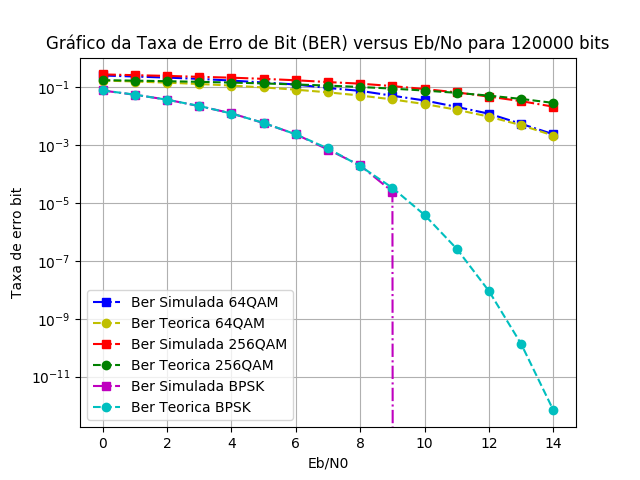
\includegraphics{certoBEROFDM.png}
    \caption{BER x SNR}
    \label{fig:my_label}
\end{figure}

Com este gráfico podemos observar que não há diferença entre o sinal com ou sem OFDM(teórico), e quanto maior o numero de bits por simbolo (bits por sim = log$_{2}$(M)), maior será a probabilidade de erro de bits. Foi escolhido essa quantidade de bits para a transmissão por causa do processamento computacional que causa colocar uma maior quantidade de bits. Podemos perceber também que com aumento do Eb/N0 a probabilidade de erro de bits diminui, isso é devido a que os bits ficam menos espalhados e mais próximos  do sinal original assim acontecendo uma menor quantidade de erros de bits. Também é possível perceber no gráfico que a quantidade de erro de cai pra zero, isso significa que não há bits suficientes para poder estimar a BER até os 15 dB de Eb/N0.




\section{References}
\cite{proakis:11}

\bibliographystyle{sbc}
\bibliography{sbc-template}
\end{document}
